\section{Introduction}

\label{sec:intro}

\begin{frame}{Problem statement}
	\only<1>
	{
	\begin{minipage}{0.75\linewidth}
		\begin{figure}
			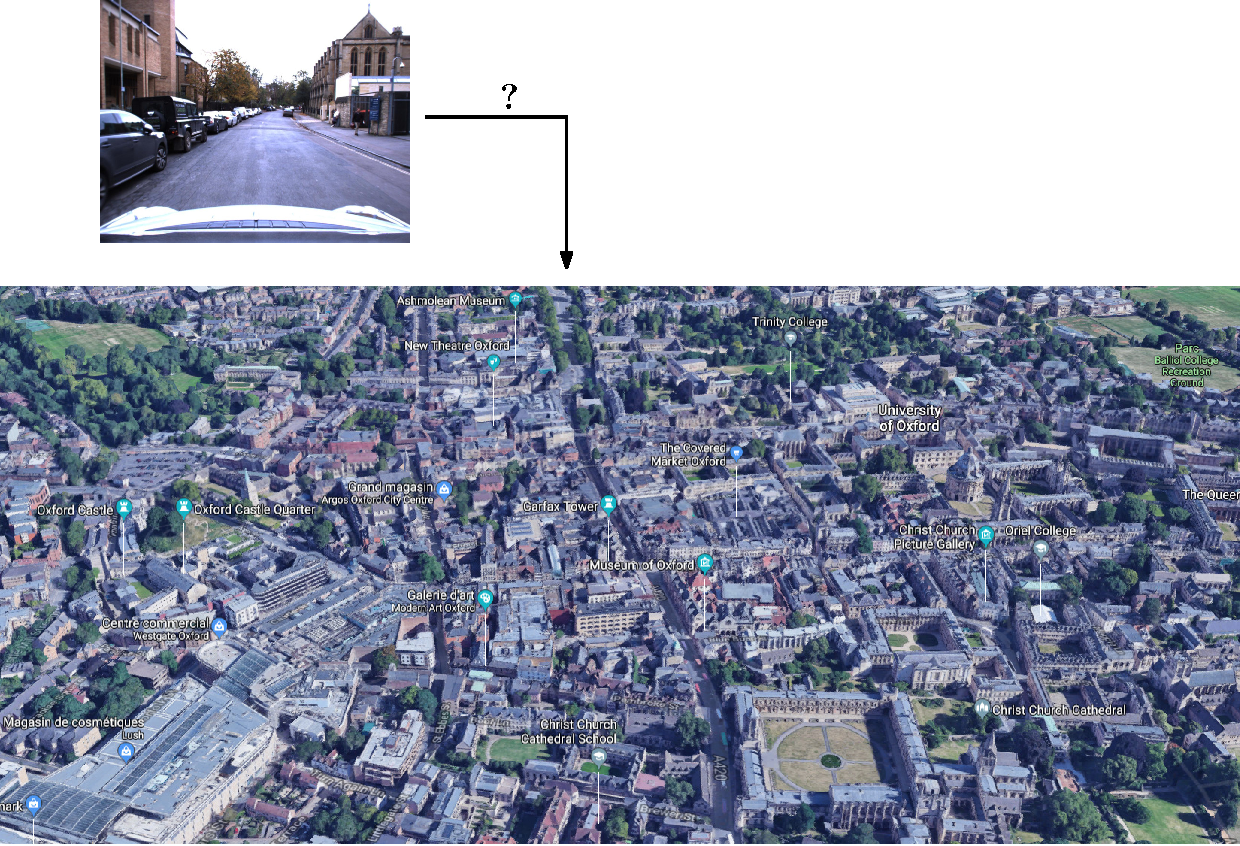
\includegraphics[width=\linewidth]{vect/intro/fig1/1}
		\end{figure}		
	\end{minipage}
	\hfill
	\begin{minipage}{0.18\linewidth}
		We aim to recover the position of an \textbf{unknown query}.	
	\end{minipage}
	}
	\only<2>
	{
	\begin{minipage}{0.75\linewidth}
		\begin{figure}
			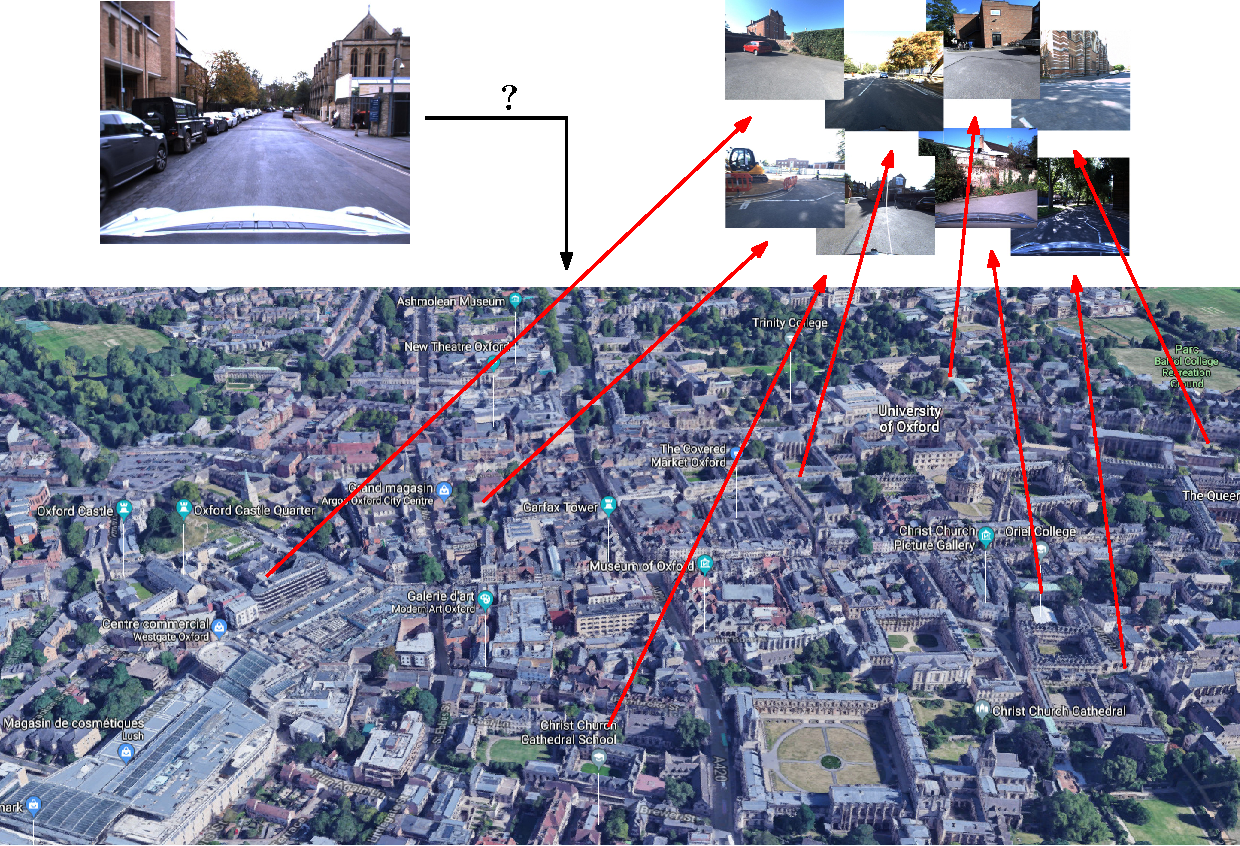
\includegraphics[width=\linewidth]{vect/intro/fig1/2}
		\end{figure}		
	\end{minipage}
	\hfill
	\begin{minipage}{0.18\linewidth}
			We have access to \textbf{geo-localized data}.
	\end{minipage}
	}
	\only<3>
	{
	\begin{minipage}{0.75\linewidth}
		\begin{figure}
			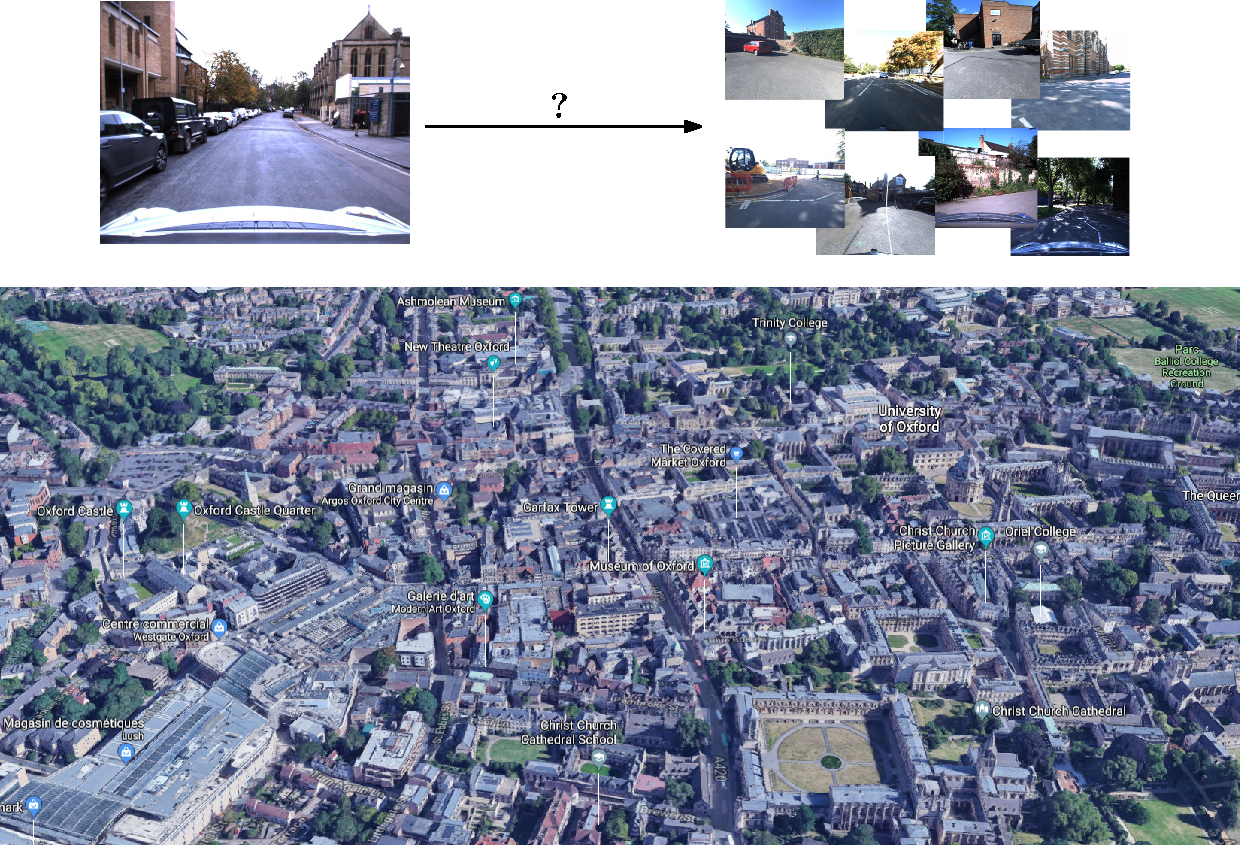
\includegraphics[width=\linewidth]{vect/intro/fig1/3}
		\end{figure}		
	\end{minipage}
	\hfill
	\begin{minipage}{0.18\linewidth}
		We caste the image localisation problem as an \textbf{image-retrieval problem}.
	\end{minipage}
	}
	\only<4>
	{
	\begin{minipage}{0.75\linewidth}
		\begin{figure}
			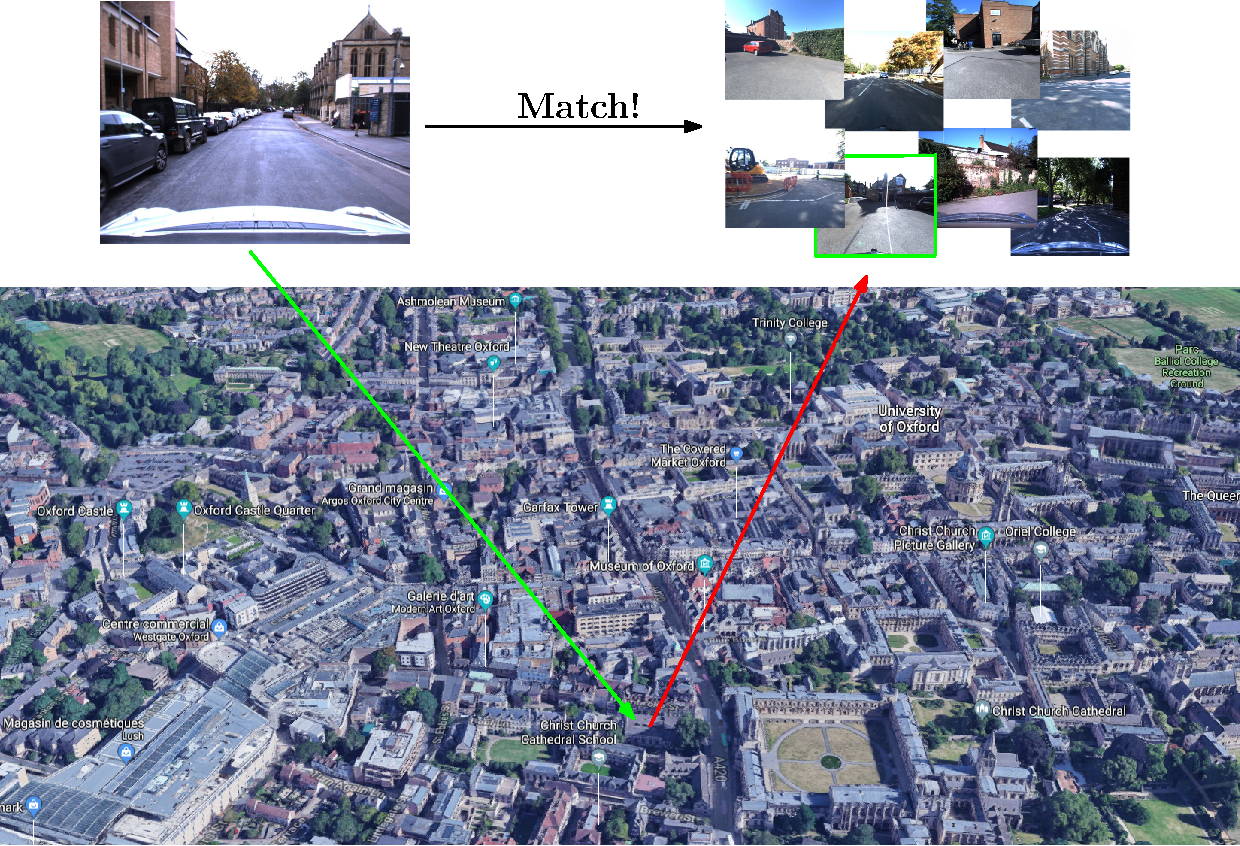
\includegraphics[width=\linewidth]{vect/intro/fig1/4}
		\end{figure}		
	\end{minipage}
	\hfill
	\begin{minipage}{0.18\linewidth}
		We transfer the position of the \textbf{retrieved candidate} to the query.
	\end{minipage}
	}
\end{frame}

\begin{frame}{Challenge in visual based localization}
	\begin{minipage}{0.75\linewidth}
		\begin{figure}
			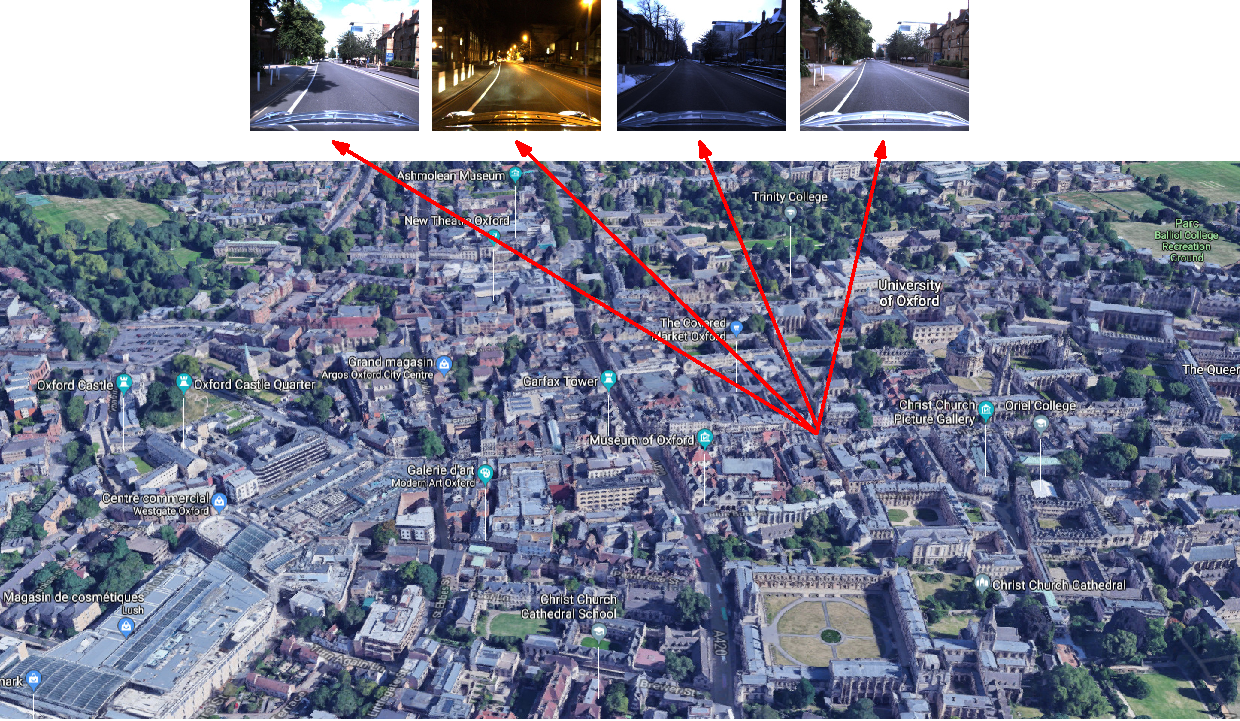
\includegraphics[width=\linewidth]{vect/intro/fig4/1}
		\end{figure}		
	\end{minipage}
	\hfill
	\begin{minipage}{0.18\linewidth}
		Drastic \textbf{visual changes} occur due to season/day-night cycles.
	\end{minipage}
\end{frame}	

\begin{frame}{Geometry to the rescue}
	\only<1>
	{
	\vfill
	\begin{figure}
		\centering
		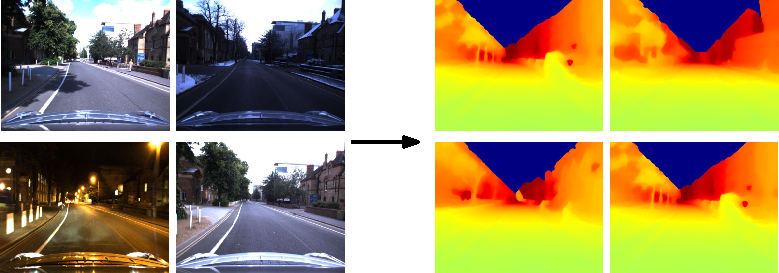
\includegraphics[width=0.8\linewidth]{vect/intro/fig4/2}
	\end{figure}
	\vfill	
	However, \textbf{geometric information} still remains the same.
	}
	\only<2>
	{
	\vfill
	\begin{figure}
		\centering
		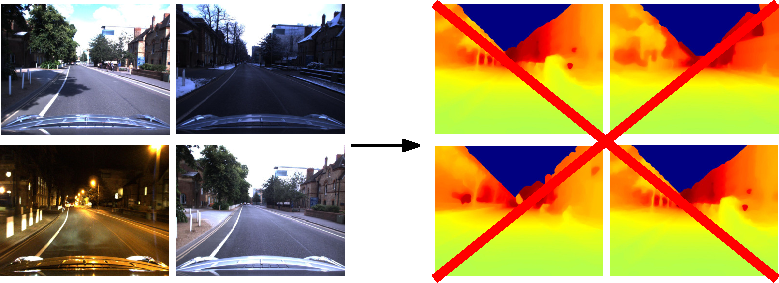
\includegraphics[width=0.8\linewidth]{vect/intro/fig4/3}
	\end{figure}
	\vfill	
	Unfortunately, geometric information is \textbf{not always available}.
	}
	\only<3>
	{
	\vfill
	\centering
	\begin{figure}
		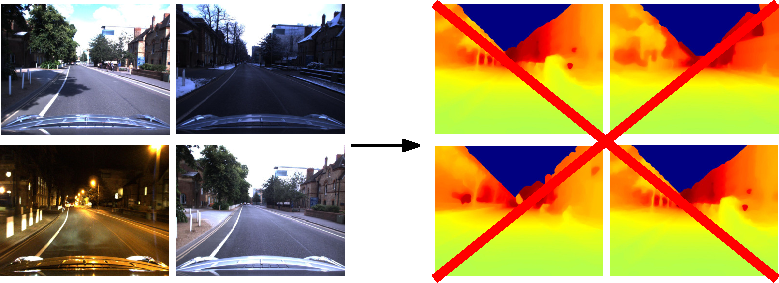
\includegraphics[width=0.6\linewidth]{vect/intro/fig4/3}
	\end{figure}
	\vfill	
	\textbf{How to use partial geometric information to improve image descriptor for localization?}
	}
\end{frame}
